% This is samplepaper.tex, a sample chapter demonstrating the
% LLNCS macro package for Springer Computer Science proceedings;
% Version 2.20 of 2017/10/04
%
\documentclass[runningheads]{llncs}
%
\usepackage{graphicx}
\usepackage[hidelinks,breaklinks=true,backref=page]{hyperref}

\usepackage[spanish]{babel}
\usepackage[utf8]{inputenc}
% Used for displaying a sample figure. If possible, figure files should
% be included in EPS format.
%
% If you use the hyperref package, please uncomment the following line
% to display URLs in blue roman font according to Springer's eBook style:
% \renewcommand\UrlFont{\color{blue}\rmfamily}

\begin{document}

%
\title{Reconocimiento de Entidades Nombradas}
%
%\titlerunning{Abbreviated paper title}
% If the paper title is too long for the running head, you can set
% an abbreviated paper title here
%
\author{Luis Ernesto Ibarra Vázquez\inst{1} \and
Luis Enrique Dalmau Coopat\inst{2}}
%
%\authorrunning{F. Author et al.}
% First names are abbreviated in the running head.
% If there are more than two authors, 'et al.' is used.
%
\institute{Universidad de La Habana, La Habana, Cuba}
%
\maketitle              % typeset the header of the contribution
%
\begin{abstract}
%The abstract should briefly summarize the contents of the paper in
%150--250 words.

%TODO Agregarle algos obre NLP solo
En este trabajo abordaremos acerca de una visión general de NLP, explicando en que se basa y los distintos modelos usados en dicha rama. Trataremos uno de los aspectos más desafiantes del NLP que es la extracción de entidades nombradas(NER).Esta consiste en la extracción y clasificación de entidades en un texto. Este documento presenta una definición del problema además de introducir los principales retos enfrentados en estos problemas y qué técnicas existen para darle una respuesta lo más acertada posible. 

\keywords{Entidades Nombradas  \and Aprendizaje de Máquina \and Procesamiento de Lenguaje Natural.}
\end{abstract}
%
%
%
\section{Introducción}

En el contexto actual con el desarrollo de las tecnologías, la explosión de información no estructurada en la web ha hecho que sea necesario un procesamiento para lograr extraer información por medios computacionales. De esto se encarga el Procesamiento de Lenguaje Natural, el cual es una rama de Inteligencia Artificial encargada de la creación de modelos y algoritmos para atacar este tipo de problemas. Una información en particular que se desea extraer en el procesamiento de textos son las entidades que más significado semántico aportan al texto, saber las entidades que se encuentran en este y cuáles son las categorías a las que pertenecen dichas entidades, en la literatura este problema se conoce como Extracción de Entidades Nombradas.

La solución de dicho problema traería consigo una manera de estructurar efectivamente muchos de estos documentos no estructurados pudiendo llegar a un estado de organización de los documentos presentes en la web agilizando diferentes tareas. En la recuperación de información se pueden usar las entidades nombradas para mejorar el resultado obtenido por los buscadores, en la medicina se pueden encontrar las relaciones existentes entre diferentes entidades creando una base de datos que pueda servir como ontología para futuras consultas.

En el documento se presenta primero las dificultades generales del Procesamiento de Lenguaje Natural. Luego se introduce el tema sobre la Extracción de Entidades Nombradas y los algoritmos usados para resolverlos además de los problemas comunes que se enfrentan a la hora de la extracción de entidades. Por último se presentan los distintos usos de la extracción de entidades en el proceamiento de documentos para la solución de distintos problemas.

\section{Procesamiento de Lenguaje Natural}

\subsection{¿Qué es el Procesamiento del Lenguaje Natural?\protect\footnote{Todo pertenece a \cite{nlp}}}
El Procesamiento del Lenguaje Natural ,como se menciona anteriormente, es el campo de conocimiento de la Inteligencia Artificial que se ocupa de investigar la manera de comunicar a las máquinas con las personas mediante el uso de lenguas naturales, como el español, el inglés o cualquier 
El Procesamiento del Lenguaje Natural, como se menciona anteriormente, es el campo de conocimiento de la Inteligencia Artificial que se ocupa de investigar la manera de comunicar a las máquinas con las personas mediante el uso de lenguas naturales, como el español, el inglés o cualquier 
otro idioma.

Las lenguas humanas pueden expresarse por escrito (texto), oralmente (voz) y también mediante signos. Naturalmente, el NLP está más avanzado en el tratamiento de textos, donde hay muchos más datos y son más fáciles de conseguir en formato electrónico.

Los audios, aunque estén en formato digital, hay que procesarlos para transcribirlos en letras o caracteres y, a partir de ahí, entender la pregunta. El proceso de respuesta es el inverso: primero se elabora la oración y luego se “sintetiza la voz”.

Por cierto, la voz artificial cada vez suena más humana, con inflexiones tonales y prosódicas que imitan la producción humana.



\subsection{Modelos para procesamiento del lenguaje natural\protect\footnote{Todo pertenece a \cite{nlp}}}

Tratar computacionalmente una lengua implica un proceso de modelación matemática. Los lingüistas computacionales se encargan de la tarea de “preparar” el modelo lingüístico para que posteriormente se implemente la modelación lingüística:
\begin{itemize}


\item{\textbf{Modelos Lógicos: gramáticas}

Los lingüistas escriben reglas de reconocimiento de patrones estructurales, empleando un formalismo gramatical concreto. Estas reglas, en combinación con la información almacenada en diccionarios computacionales, definen los patrones que hay que reconocer para resolver la tarea (buscar información, traducir, etc.).

Estos modelos lógicos pretenden reflejar la estructura lógica del lenguaje y surgen a partir de las teorías de N. Chomsky en los años 50.} 


\item{\textbf{Modelos probabilísticos del lenguaje natural: basados en datos}

La aproximación es a la inversa: los lingüistas recogen colecciones de ejemplos y datos (corpus) y a partir de ellos se calculan las frecuencias de diferentes unidades lingüísticas (letras, palabras, oraciones) y su probabilidad de aparecer en un contexto determinado. Calculando esta probabilidad, se puede predecir cuál será la siguiente unidad en un contexto dado, sin necesidad de recurrir a reglas gramaticales explícitas.

Es el paradigma de “aprendizaje automático” que se ha impuesto en las últimas décadas en Inteligencia Artificial: los algoritmos infieren las posibles respuestas a partir de los datos observados anteriormente en el corpus.}
\end{itemize}

\subsection{Componentes del procesamiento del lenguaje natural\protect\footnote{Todo pertenece a \cite{nlp}}}

A continuación, vemos algunos de los componentes del procesamiento del lenguaje natural. No todos los análisis que se describen se aplican en cualquier tarea de NLP, sino que depende del objetivo de la aplicación.

\begin{itemize}
    \item \textbf{Análisis morfológico o léxico}. Consiste en el análisis interno de las palabras que forman oraciones para extraer lemas, rasgos flexivos, unidades léxica compuestas. Es esencial para la información básica: categoría sintáctica y significado léxico.
    \item \textbf{Análisis sintáctico}. Consiste en el análisis de la estructura de las oraciones de acuerdo con el modelo gramatical empleado (lógico o estadístico).
    \item \textbf{Análisis semántico}. Proporciona la interpretación de las oraciones, una vez eliminadas las ambigüedades morfosintácticas.
    \item \textbf{Análisis pragmático}. Incorpora el análisis del contexto de uso a la interpretación final. Aquí se incluye el tratamiento del lenguaje figurado (metáfora e ironía) como el conocimiento del mundo específico necesario para entender un texto especializado.
\end{itemize}


 %HINT Características del procesamiento del Lenguaje Natural según su estructura y especificidades de cada idioma
 
\subsection{Dificultades en el procesamiento}
 
En cuanto al NLP podemos darnos cuenta rápidamente de varios problemas que surgen dada la inmensa cantidad de diferencias entre los distintos idiomas existentes en nuestro planeta. No es igual el uso de pronombres en todas las lenguas, incluso en algunas estos se encuentran incluidos en la palabra a la que refieren como se dan los casos en el idioma alemán. Muchos otros idiomas tienen distintas estructuras y orden a pesar de que hayan muchas características comunes como el sujeto y el predicado.

Incluso podemos tener en cuenta que hay palabras existentes en algunos idiomas que en otros no, al igual que contracciones y palabras nativas de la jerga local. Además, no siempre los organismos ofciciales encargados de cada lengua se encuentran al día con la evolución de su respectivo idioma.


\section{Entidad nombrada}

La definición de entidad nombrada se puede ver formalmente en los designadores rígidos\cite{rigid_designator}, los cuales son términos que designan un mismo elemento en todos los mundos posibles en que ese elemento existe. Generalmente incluyen nombres propios y términos científicos tales como nombre de sustancias, elementos químicos. Esta definición es solo un punto de partida para el análisis de las entidades ya que se puede relajar  para abarcar más elementos como por ejemplo, las expresiones temporales y numéricas, como cantidades de dinero y unidades de medida, se toman como entidades nombradas. 

\subsection{Ejemplos}

\begin{itemize}

\item Universidad de La Habana: Entidad nombrada
\item universidad: No es una entidad nombrada, puede representar entidades diferentes.
\item Facultad de Matemática y Computación de la Universidad de La Habana: Entidad nombrada
\item UH: Entidad nombrada
\item \$2: Entidad nombrada
\end{itemize}

\subsection{Problemas}

En los ejemplos anteriores se evidencian algunos de los problemas que tiene la extracción de entidades nombradas. En el \emph{Universidad de La Habana} se presentan dos entidades \emph{solapadas}, la entidad completa como organización y La Habana como lugar, sin embargo la más correcta es la de universidad como organización. Para mitigar este problema las entidades nombradas se toman como una sucesión de tokens que no se solapan. Otro problema reflejado en el ejemplo de \emph{universidad} es la falta de la capacidad de inferir a la entidad a la que se refieren, lo cual puede traer que se pierda mucha información en el análisis del texto. Además del problema de solapamiento, se encuentra el problema de las entidades anidadas. En el ejemplo de \emph{Facultad de Matemática y Computación de la Universidad de La Habana} se presentan dos entidades las cuales tienen sentido de manera independiente \emph{Facultad de Matemática y Computación} y \emph{Universidad de La Habana}, ver cuando estas entidades van juntas o separadas constituye un problema en la extracción de entidades.

\section{Categorías}

Las categorías son grupos a los que las entidades nombradas pertenecen. La variedad de estos grupos y su interrelacción entre ellos está dada principalmente por el contexto del problema a tratar. Las principales categorías son: \textbf{persona}, \textbf{organización} y \textbf{lugar}, estas se pueden encontrar en todo texto independientemente del tema que traten aunque existen varias definiciones de categorías llegando algunas incluso a formar jerarquías. Las categorías también pueden crearse en dependencia del contexto en que se vaya a procesar el texto, especializándolas más para lograr extraer información más exactas, esto ocurre principalmente en el campo de la química y la biología en la cual los nombres de las sustancias se califican en categorías afines. Un ejemplo de una definición general jerárquica se encuentra en la versión de \cite{sekine} que cuenta con unos 200 subtipos.

\subsection{Ejemplos}

\begin{itemize}

\item Universidad de La Habana: Organización
\item La Habana: Lugar
\item Luis Ernesto: Persona

\end{itemize}

\subsection{Problemas}

La asignación de categorías a las entidades presentan varios problemas. Uno de ellos es seleccionar el conjunto de categorías en las que se va a mover las entidades nombradas, teniendo mucho peso el contexto del problema, por ejemplo si se está analizando un conjunto de datos sobre música, podrían ser relevantes tener las categorías de disquera, músico, etc, las cuales extraigan información relevante de los documentos. Un problema común es la propia ambigüedad del lenguaje, por ejemplo, en el caso de que exista una organización y un lugar llamados iguales se complica la clasificación de este ya que dado el contexto podría ser cualquiera de las dos. Por ejemplo, se tienen las oraciones: \emph{said Harry You, CEO of HearingPoint} y \emph{For this year’s second quarter, You said the
company’s} \cite{semi_sup_for_ner}, en estos campos ambos \emph{You} corresponden al nombre de una misma persona, pero el segundo se puede clasificar como un pronombre personal también, que en cuyo caso no sería una entidad nombrada.

\section{Extracción de Entidades Nombradas (NER)}

Dada las definiciones anteriores el problema de Reconocimiento de Entidades Nombradas se puede definir como la extracción y clasificación de las entidades nombradas de un texto. Como dice en la definición, el problema se divide en dos partes fundamentales: extracción y clasificación.

\subsection{Extracción de entidades}

La extracción de entidades consiste en extraer del texto las entidades existentes en él ya anotadas con diferentes metadatos como la parte de oración que representa, la posición dentro de una entidad, entre otras. En este proceso intervienen dos etapas que se interrelacionan entre sí: \emph{chunking}\cite{chunking} y \emph{Part-of-Speech (POS) Tagging}\cite{postag}.

\subsubsection{POS Tagging}

El objetivo de este subproblema es anotar una secuencia de tokens con la parte de la oración que representa, estas partes dependen del idioma y del conjunto seleccionado por el personal que realice el software en dependencia de la necesidad del programa. En este caso nos enfocaremos en el idioma inglés en el cual existen 9 tipos de POS importantes de los que sobrealen: sustantivo, verbo, adjetivo, preposición, pronombre y adverbio, los cuales son horizontales a la mayoría de los lenguajes. En la literatura existen otros conjuntos de etiquetas basados en las partes mencionadas anteriores pero que agregan otros datos como si se está en plural o singular, tiempo del verbo etc, entre estos se encuentran:

\begin{itemize}
\item Penn Treebank \cite{pennpostag}
\item Brown Corpus \cite{brownpostag}
\end{itemize}

Por ejemplo la frase \emph{I study at University of Havana} produce la siguiente salida: \emph{I|PRON study|VERB at|ADP University|PROPN of|ADP Havana|PROPN}.

Para resolver este problema se han ideado diferentes aproximaciones:

\begin{itemize}

\item Expersiones regulares: Las expresiones regulares son usadas principalemente a la hora de anotar cantidades de dinero o entidades que empiezan con honoríficos como Sr, Dr, MsC, entre otras en las cuales existe una alta probabilidad de que la anotación sea correcta.

\item Aprendizaje de máquina: Se han usado diferentes algoritmos para este problema como SVM, perceptron, nearest-neighbor, llegando a una precisión superior del 95\% \cite{postag}

\item Modelos ocultos de Markov (Hidden Marcov Models HMM): En el caso más simple este modelo se puede ver como un grafo dirigido en el cual los estados representan las partes de la oración y las aristas representan las posibles transiciones del estado actual al siguiente, estas aristas están ponderadas con la probabilidad de cuál es el estado siguiente. El estado no observable representa la etiqueta POS y el estado observable representa el token actual \cite{hmm}.

\end{itemize}

\subsubsection{Chunking}

%Esta etapa del proceso ocurre luego del POS-tagging y se encarga de agrupar los tokens antodados del POS en partes más significativas de la oración creando un árbol cuya raíz es el texto y las hojas los tokens anotados. Siguiendo el ejemplo: \emph{I|PRON study|VERB at|ADP University|PROPN of|ADP Havana|PROPN} se convierte en Fig.\ref{syntaxtree}
%
%\begin{figure}
%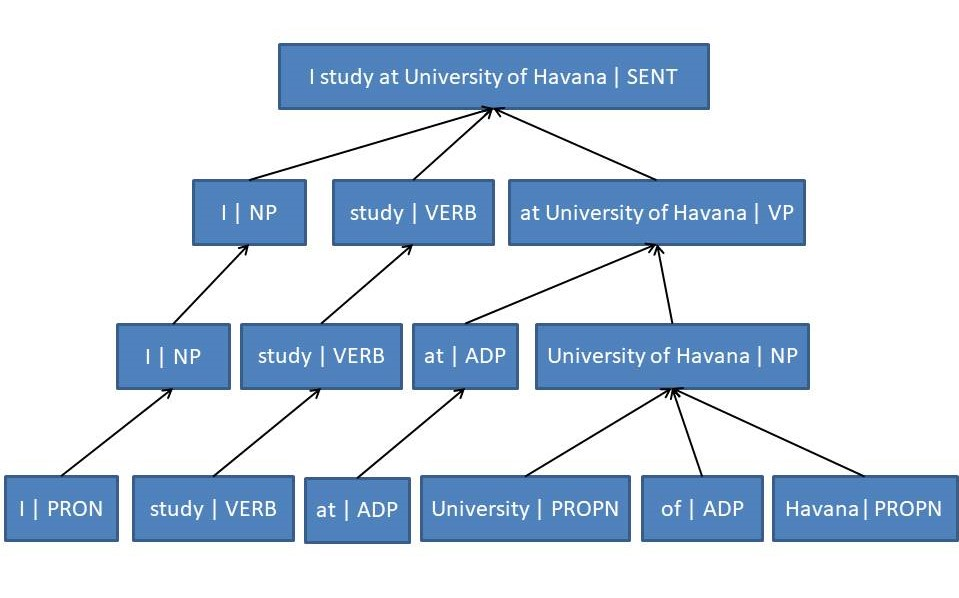
\includegraphics[width=\textwidth]{syntaxtree.jpg}
%\caption{Árbol de sintaxis} \label{syntaxtree}
%\end{figure}

%Sobre este árbol se realizan diferentes algoritmos para la extracción de entidades nombradas:

Esta etapa se puede ver como un problema de segmentación en la cual se quiere particionar los tokens, generalmente anotados previemente con las etiquetas POS, en conjuntos que identifiquen las entidades nombradas.

\begin{figure}
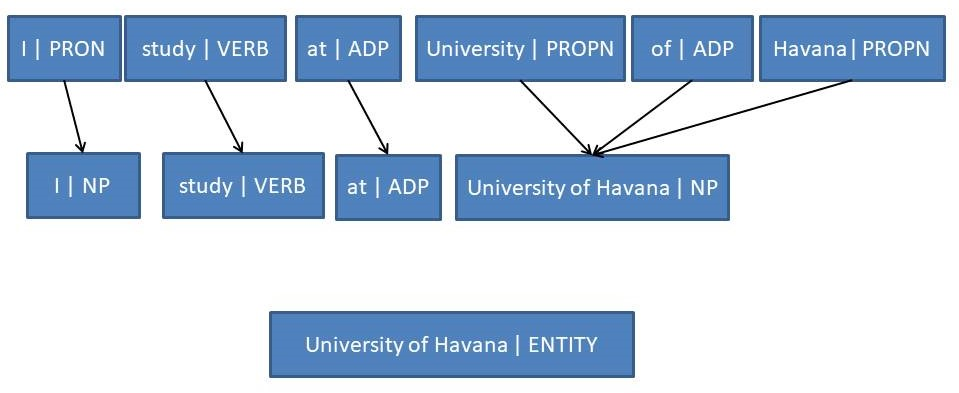
\includegraphics[width=\textwidth]{namedentity.jpg}
\caption{Chunking} \label{chunkingfig}
\end{figure}

Para lograr esta anotación se utilizan varias aproximaciones:

\begin{itemize}

\item Gramáticas: Se les da gramáticas en las que los términos finales son las anotaciones de la parte de la
oración y luego son parseadas en dependencia de estas. Algunos parsers proveen la capacidad de 
tener expresiones regulares en su interior aumentando la expresividad \cite{nltkgrammar}

\item Aprendizaje de Máquina: Generalmente se realiza un aprendizaje supervisado mediante un conjunto de datos, las entradas del conjunto de datos varían pero las más simples es una tupla \emph{(palabra, IOB tag)}.  IOB es una anotación que va acompañada en cada token y representa si una parte esta dentro (In), fuera (Outside) o inicio (Beginning) de un pedazo o entidad.

\end{itemize}

\subsection{Clasificación de entidades}

Esta parte del problema es la encargada de clasificar todas las entidades extraídas del texto en las diferentes categorías seleccionadas. La más ampliamente usada es aprendizaje de máquina, en esta se utiliza el aprendizaje supervisado para elaborar una función que dada un texto anotado devuelva las categorías a las que pertenecen estas, entre los algoritmos que se pueden utilizar encuentran:

\begin{itemize}

\item K-Nearest Neighbor
\item Árboles de decisión
\item Naive Bayes
\item Random Forest
\item Regresión Logística (Con estrategias para soportar múltiples clases)
\item SVM (Con estrategias para soportar múltiples clases)

\end{itemize}

Otra vía más directa de clasificación de entidades es el uso de bases de conocimiento. Estas se pueden usar para buscar las entidades directamente y anotarlas en dependencia de dónde se encontró. Además con el uso de expresiones regulares es posible clasificar las entidades, por ejemplo: expresiones como \emph{Dr.} y \emph{MSc.} son comunmente usados en personas.

\subsection{Software}

Para la extracción de entidades nombradas existen varios softwares, entre los más importantes se presentan:

\begin{itemize}

\item spaCy \cite{spacy_nlp}
\item Standford NLP \cite{standford_nlp}
\item GATE \cite{gate_nlp}
\item Apache OpenNLP \cite{open_nlp}

\end{itemize}

Todas estas herramientas, además de reconocimiento de entidades, permiten realizar diferentes operaciones orientadas al procesamiento de lenguaje natural.

\section{Problemas Generales de NER}

La extracción de entidades nombradas incurren en diferentes problemas uno de ellos está relacionado principalmente con el corpus usado para el entrenamiento del sistema. La creación de corupus de manera manual es uno de los principales problemas que tiene el aprendizaje supervisado, rango en el cual caen la mayoría de los algoritmos vistos. Para la creación del corpus, lingüistas necesitan dedicar varias horas en esta tarea para poder lograr una cantidad relevante de documentos anotados con calidad. En este aspecto se han hecho esfuerzos en métodos de aprendizaje semisupervisado que asistan en la tarea. %TODO Agreagr los esfuerzos realizados.

En general los corpus existentes se han entrenado en un ambiente relativamente cerrado y uniforme, por ejemplo, Wikipedia, periódicos, artículos científicos, esto tiene como consecuencia que si se usa este sistema en un ambiente no relacionado o estructurado de manera similar el rendimiento baje. Un ejemplo clásico en el cual esto ocurre es en Twitter, debido a la gran cantidad de temas en los que se habla, la cantidad limitada de 140 caracteres, la ausencia de reglas para escribir,  entre otros elementos hace que los NER se desempeñen de manera pobre. Este problema es abordado en \cite{tweeter}, en este artículo sus escritores lograron reducir los errores en el POS hasta un 41\% con respecto al Standford POS Tagger y logrando una métrica F1 final de 0.59 en comparación con 0.29 del Standford NER. 

Otro problema relacionado con el corpus es el inherente error humano y la propia ambigüedad del lenguaje, esto hace que en oraciones con la misma sintaxis y semántica las anotaciones difieran por errores humanos, pudiendo llevar en el peor de los casos a variar el rendimiento del sistema en un 5\% \cite{posdecisiontree}. Aunque en general los anotadores humanos son hasta ahora la manera más fiable de obtener información anotada correctamente, esto requiere del trabajo manual de estos lo cual se hace en muchos casos impracticable debido al gran volumen de datos que se procesa hoy en día.

\section{Usos}

La extracción de entidades nombradas puede ser utilizada para darle solución a diferentes problemas. Uno de ellos es que este procedimiento es el primer paso para la creación de un sistema de extracción de relaciones en los documentos, en los cuales una vez se tengan las entidades con sus clasificaciones es necesario buscar las diferentes relaciones que existen entre ellos para finalmente crear una base de datos estructurada con esta información. Un ejemplo de lo anterior se evidencia en el texto \emph{Facebook compró WhatsApp}, en el cual se evidencian dos organizaciones \emph{Facebook} y \emph{WhatsApp} y la relación \emph{comprar}.

En la recuparación de información la extracción se puede usar para mejorar la búsqueda. Por ejemplo teniendo un corpus anotado con las entidades que aparecen en él, la recuperación se puede realizar sobre estas, reduciendo la cantidad de términos necesarios para realizar la búsqueda enfocándose solo en ellas, que son las que aportan el mayor significado semántico al texto. Además estas anotaciones se pueden usar en la clasificación del texto acorde a su temática y con esto último es posible realizar búsquedas más precisas.

En la construcción de un sistema de atención al cliente la extracción de entidades puede ayudar a dirigir la queja del cliente al departamento que se le asocie automáticamente. Esto es posible ya que en estos mensajes generalmente están los distintos productos y lugares en dónde se detectó el problema, pudiendo extraer esta información y posteriormente enviándole el mensaje al departamento asignado. Por ejemplo: \emph{Etecsa, la conexión en La Habana está terrible en el horario de 8 a 11 de la noche}, en el mensaje anterior la queja se enviará al departamento de Etecsa en La Habana.

Otras áreas en las que se usa la extracción de entidades son: \cite{ner_thesis}

\begin{itemize}

\item Traducción de máquina
\item Sistemas de Pregunta y Respuesta
\item Creación Automática de Resúmenes
\item Análisis de Sentimiento
\item Creación de clústers de documentos

\end{itemize}

\section{Conclusiones}

%TODO Poner conclusiones

Podemos afirmar entonces que el Reconocimiento de Entidades Nombradas es una herramienta de mucha utilidad y que nos facilita resolver muchos de nuestros problemas actuales. Llegar a un punto de dar una consulta a la maquina en lenguaje natural y que esta devuelva lo que queremos es algo que no tiene precio. Pero aún es muy pronto para este campo del NLP que a pesar de tener 50 años de investigación, el lenguaje natural en su expresión más innata como vimos en el caso de las redes sociales sigue siendo un gran desafío para la ciencia al que cada vez estamos más cerca de resolver.

%\subsubsection{Sample Heading (Third Level)} Only two levels of
%headings should be numbered. Lower level headings remain unnumbered;
%they are formatted as run-in headings.
%
%\paragraph{Sample Heading (Fourth Level)}
%The contribution should contain no more than four levels of
%headings. Table~\ref{tab1} gives a summary of all heading levels.
%
%\begin{table}
%\caption{Table captions should be placed above the
%tables.}\label{tab1}
%\begin{tabular}{|l|l|l|}
%\hline
%Heading level &  Example & Font size and style\\
%\hline
%Title (centered) &  {\Large\bfseries Lecture Notes} & 14 point, bold\\
%1st-level heading &  {\large\bfseries 1 Introduction} & 12 point, bold\\
%2nd-level heading & {\bfseries 2.1 Printing Area} & 10 point, bold\\
%3rd-level heading & {\bfseries Run-in Heading in Bold.} Text follows & 10 point, bold\\
%4th-level heading & {\itshape Lowest Level Heading.} Text follows & 10 point, italic\\
%\hline
%\end{tabular}
%\end{table}
%
%
%\noindent Displayed equations are centered and set on a separate
%line.
%\begin{equation}
%x + y = z
%\end{equation}
%Please try to avoid rasterized images for line-art diagrams and
%schemas. Whenever possible, use vector graphics instead (see
%Fig.~\ref{fig1}).
%
%\begin{figure}
%\includegraphics[width=\textwidth]{userPhoto.jpg}
%\caption{A figure caption is always placed below the illustration.
%Please note that short captions are centered, while long ones are
%justified by the macro package automatically.} \label{fig1}
%\end{figure}
%
%\begin{theorem}
%This is a sample theorem. The run-in heading is set in bold, while
%the following text appears in italics. Definitions, lemmas,
%propositions, and corollaries are styled the same way.
%\end{theorem}
%%
%% the environments 'definition', 'lemma', 'proposition', 'corollary',
%% 'remark', and 'example' are defined in the LLNCS documentclass as well.
%%
%\begin{proof}
%Proofs, examples, and remarks have the initial word in italics,
%while the following text appears in normal font.
%\end{proof}
%For citations of references, we prefer the use of square brackets
%and consecutive numbers. Citations using labels or the author/year
%convention are also acceptable. The following bibliography provides
%a sample reference list with entries for journal
%articles~\cite{ref_article1}, an LNCS chapter~\cite{ref_lncs1}, a
%book~\cite{ref_book1}, proceedings without editors~\cite{ref_proc1},
%and a homepage~\cite{ref_url1}. Multiple citations are grouped
%\cite{ref_article1,ref_lncs1,ref_book1},
%\cite{ref_article1,ref_book1,ref_proc1,ref_url1}.
%
% ---- Bibliography ----
%
% BibTeX users should specify bibliography style 'splncs04'.
% References will then be sorted and formatted in the correct style.
%
% \bibliographystyle{splncs04}
% \bibliography{mybibliography}
%
\begin{thebibliography}{8}
%\bibitem{ref_article1}
%Author, F.: Article title. Journal \textbf{2}(5), 99--110 (2016)
%
%\bibitem{ref_lncs1}
%Author, F., Author, S.: Title of a proceedings paper. In: Editor,
%F., Editor, S. (eds.) CONFERENCE 2016, LNCS, vol. 9999, pp. 1--13.
%Springer, Heidelberg (2016). \doi{10.10007/1234567890}
%
%\bibitem{ref_book1}
%Author, F., Author, S., Author, T.: Book title. 2nd edn. Publisher,
%Location (1999)
%
%\bibitem{ref_proc1}
%Author, A.-B.: Contribution title. In: 9th International Proceedings
%on Proceedings, pp. 1--2. Publisher, Location (2010)

\bibitem[ICCNLP]{nlp}\url{https://www.iic.uam.es/inteligencia/que-es-procesamiento-del-lenguaje-natural/}.Accedido 24 de abril 2022

\bibitem[SEKINE]{sekine}New York University, Natural Language Processing Section, \url{https://nlp.cs.nyu.edu/ene/version7\_1\_0Beng.html}. Accedido 13 de abril 2022

\bibitem[RIGID]{rigid_designator}
Wikipedia, \url{https://en.wikipedia.org/wiki/Rigid\_designator}. Accedido 13 de abril 2022

\bibitem[SHALLOW]{chunking}
Wikipedia, \url{https://en.wikipedia.org/wiki/Shallow\_parsing}. Accedido 12 de abril 2022

\bibitem[POSTAG]{postag}
Wikipedia, \url{https://en.wikipedia.org/wiki/Part-of-speech\_tagging}. Accedido 13 de abril 2022

\bibitem[PENNPOSTAG]{pennpostag}
University of Pensilvania Departament of Linguistics, \url{https://www.ling.upenn.edu/courses/Fall\_2003/ling001/penn\_treebank\_pos.html}. Accedido 13 de abril 2022

\bibitem[TOWARDS]{hmm}
Towards Data Science, \url{https://towardsdatascience.com/part-of-speech-tagging-for-beginners-3a0754b2ebba}. Accedido 13 de abril 2022

\bibitem[BROWN]{brownpostag}
Wikipedia, \url{https://en.wikipedia.org/wiki/Brown\_Corpus\#Part-of-speech\_tags\_used}. Accedido 13 de abril 2022

\bibitem[LNCS]{ref_url1}
LNCS Homepage, \url{http://www.springer.com/lncs}. Last accessed 4 Oct 2017

\bibitem[NLTK]{nltkgrammar}
Steven Bird, Ewan Klein, and Edward Loper: Natural Language Processing with Python. Online Edition. \url{https://www.nltk.org/book/ch07.html}

\bibitem[TWITTER]{tweeter}
Alan Ritter, Sam Clark, Mausam and Oren Etzioni: Named Entity Recognition in Tweets:
An Experimental Study. University of Washington Seattle, WA 98125, USA

\bibitem[POSDT]{posdecisiontree}
Lluís Màrquez i Villodre: Part-of-speech Tagging: A Machine Learning Approach based on Decision Trees. Departament de Llenguatges i Sistemes Informàtics de la Universitat Politècnica de Catalunya, Barcelona (1999)

\bibitem[STDFNLP]{standford_nlp}
Standford NLP, \url{https://stanfordnlp.github.io/CoreNLP/index.html}. Accedido 23 de abril de 2022

\bibitem[SPCYNLP]{spacy_nlp}
Standford NLP, \url{https://spacy.io/}. Accedido 23 de abril de 2022

\bibitem[GATENLP]{gate_nlp}
Standford NLP, \url{https://gate.ac.uk/}. Accedido 23 de abril de 2022

\bibitem[OPENNLP]{open_nlp}
Apache OpenNLP, \url{https://opennlp.apache.org/}. Accedido 23 de abril de 2022

\bibitem[NERUSE1]{ner_uses_1}
Towards Data Science, \url{https://towardsdatascience.com/named-entity-recognition-applications-and-use-cases-acdbf57d595e}. Accedido 23 de abril de 2022

\bibitem[SSFNER]{semi_sup_for_ner}
Wenhui Liao, Sriharsha Veeramachaneni: A Simple Semi-supervised Algorithm For
Named Entity Recognition. In: 9th International Proceedings
on Proceedings, pp. 1--2. Publisher, Location (2010)

\bibitem[NERTHS]{ner_thesis}
Ing. Michal Konkol: Named Entity Recognition, pp. 1--2. University of West Bohemia, Faculty of Applied Sciences, Department of Computer Science and Engineering (2015)


\end{thebibliography}
\end{document}
